\documentclass{article}

\setlength{\parindent}{0pt}

\usepackage{fullpage}
\usepackage{graphicx}

\def\Nat{{\rm I\kern-.17em N}}
\def\SFF{\hbox{I\kern-.09em\hbox{I}}}
\newcommand\Bezier{B\'{e}zier }

\newcommand\projecttitle{3D Nature Environment with Procedurally Generated Terrain and Trees}
\newcommand\myname{Liam Ozog}
\newcommand\myuserid{lozog}
\newcommand\mystudentid{20515121}

\begin{document}

\begin{minipage}[t]{3in}
{\huge \bf 
	\projecttitle 
}

\medskip
Name: \myname \\ 
User ID: \myuserid \\ 
Student ID: \mystudentid 
\end{minipage}
\hfill
\begin{minipage}[t]{3in}
%%%% Use the first of these if your image is wider than tall; use the
%%%% second if your image is taller than it is wide.
\vspace{0pt}
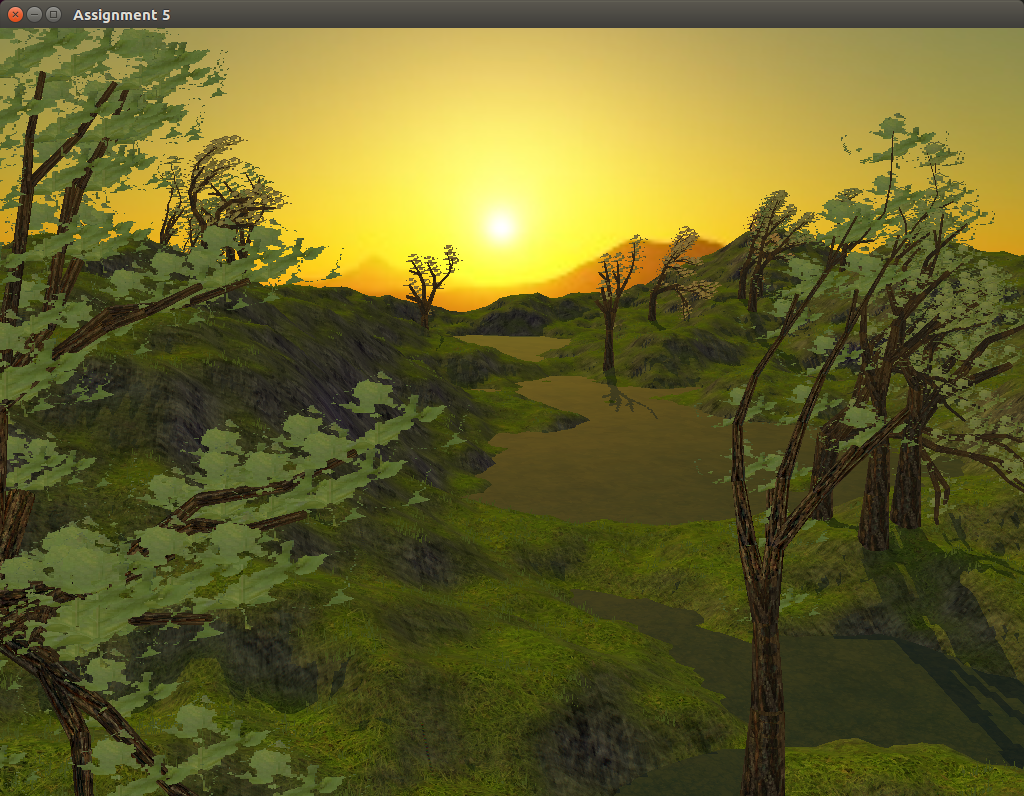
\includegraphics[width=3in]{screenshot.png}   %%%% Change file.png to your image
% \includegraphics[height=2in]{image2-FRONT.png}   %%%% Change file.png to your image
\end{minipage}


\subsection*{Artistic Merit (Polish/Artistry/Humour)}
\vfill
\subsection*{Technical Merit (Algorithms/User Interface/Graphics Techniques)}
\vfill
\subsection*{Difficulty}
\vfill
\subsection*{Code/Documentation/Demo}
\vfill
\subsection*{Mark}
\begin{center}
\begin{tabular}{lr}
Objective Mark: &~~/10\\
Subjective Mark: &~~/6\\
\hline
Total &~~/16
\end{tabular}
\end{center}

\newpage

{\huge \bf 
	\projecttitle 
}

\medskip
Name: \myname \\ 
User ID: \myuserid \\ 
Student ID: \mystudentid 

\bigskip
{\Large Objectives}

\hrule
\begin{description}
        \item[\_\_\_ 1:]
          UI: Implement a first-person camera with associated controls to allow navigation of the scene, including movement in 3 axes, speed adjustment, and camera rotation.

        \item[\_\_\_ 2:]
		  Modelling: Add a skybox to the scene using cube mapping.

        \item[\_\_\_ 3:]
		  Implement reflections for water using OpenGL's stencil buffer.
			
        \item[\_\_\_ 4:]
		  Generate a pseudo-random terrain heightmap with Perlin noise.

        \item[\_\_\_ 5:]
		  Add grass to the scene using billboards to create the illusion of many blades of grass.

        \item[\_\_\_ 6:]
	      Add texture to the ground and foliage using texture mapping.

        \item[\_\_\_ 7:]
		  Use L-systems to procedurally generate trees.

        \item[\_\_\_ 8:]
		  Implement shadows using a depth map stored in an OpenGL frame buffer.

        \item[\_\_\_ 9:]
		  Implement bloom using framebuffers and Gaussian blur.

        \item[\_\_\_ 10:]
		  Objective ten. Use a "screen-door" effect to simulate alpha transparency for grass.

\end{description}

\hrule

\end{document}
